% ===
%
% Official LaTeX seminar report template of the
% Chair for AI Methodology (AIM)
% RWTH Aachen University, Aachen, Germany
%
% Author: Jakob Bossek (bossek@aim.rwth-aachen.de)
%
% AIM website: https://aim.rwth-aachen.de/
%
% ===

% The 'review' option activates line numbering
\documentclass[review]{AIM_report}

% includes/preamble.tex is the right place to add new packages etc.
% tables
\RequirePackage{booktabs}
\RequirePackage{colortbl}
\RequirePackage{multicol}
\RequirePackage{multirow}
\RequirePackage{xspace}
\RequirePackage[final]{pdfpages}

% \smiley{} and \frowney{}
\RequirePackage{wasysym}

% quotation
\RequirePackage{csquotes}


% import commenting macros
%% commenting macros

% use this to hide larger blocks of material:
\usepackage{xcolor}
\usepackage{amsmath,amssymb}

% Define colors for authors
\definecolor{janecolor}{rgb}{0.2,0.6,0.6}
\definecolor{johncolor}{rgb}{0,0.7,0}

% Define colors for general macros
\definecolor{todocolor}{rgb}{0.9,0.1,0.1}
\definecolor{changedcolor}{rgb}{0.42,0.27,0.57}
\definecolor{addedcolor}{rgb}{0.867,0.176,0.361}

% General comment macro
\newcommand{\nbc}[3]{
    {\colorbox{#3}{\bfseries\sffamily\scriptsize\textcolor{white}{#1}}}
    {\textcolor{#3}{\sf\small$\blacktriangleright$\textit{#2}$\blacktriangleleft$}}
}
  
% Define individual comments for authors
\newcommand{\jane}[1]{\nbc{Jane}{#1}{janecolor}}
\newcommand{\john}[1]{\nbc{John}{#1}{johncolor}}

% Define general helper macros
\newcommand{\todo}[1]{\nbc{TODO}{#1}{todocolor}}
\newcommand{\changed}[1]{\nbc{CHANGED}{#1}{changedcolor}}
\newcommand{\added}[1]{\nbc{ADDED}{#1}{addedcolor}}

\newcommand{\redacted}[1]{\emph{[anonymized for review]}}
%\renewcommand{\redacted}[1]{#1}

% Use this to temporarily hide reviewing comments, todos, etc.:
%  \renewcommand{\jane}[1]{}
%  \renewcommand{\john}[1]{}

% Use this to make "changed" items appear normal:
%\renewcommand{\changed}[1]{#1}
%\renewcommand{\added}[1]{#1}
%\renewcommand{\todo}[1]{}

%% end commenting macros


% metadata
\title{Your Topic Title (Title Abbreviation)}
\subtitle{Seminar Name}
\author{Jane Doe (123456) \and John Doe (654321)}

\institute{RWTH Aachen University, Germany\\
\email{$\{$jane.doe, john.doe$\}$@rwth-aachen.de}}

% source file(s) with bibliography entries
\addbibresource{bib.bib}

\begin{document}

\maketitle

\section{Introduction}

We use the \LaTeX{} package \texttt{biblatex} for citations. Sample citation:~\cite{HutterEtAl2009}. You can also use full citations: \fullcite{HBPSTK2021TSPnormalization}

You are free to use British, American, Canadian or Australian English, but whatever you choose should be used consistently.
As Europeans, we recommend the use of British English (which is also well supported by spell and grammar checkers).

\section{Notes}

\begin{itemize}
  \item In our seminars we usualy use abbreviations to quickly identify certain topics, e.g., \textbf{NAS-1} for some kind of \emph{\underline{N}eural \underline{A}rchitecture \underline{S}earch} related topic. Please add this abbreviation into the title of your report in parenthesis after the full title.
  \item Please add your full names and your matriculation number in the \verb|\author{}| field.
\end{itemize}

\section{Figures and tables}

Figure~\ref{fig:sample_image} shows a sample image and Table~\ref{fig:sample_table} shows an exemplary table. Use the \texttt{booktabs} package to design nice tables. Avoid vertical lines whenever possible. We recommend to take a look at the presentation \href{https://people.inf.ethz.ch/markusp/teaching/guides/guide-tables.pdf}{Small Guide to Making Nice Tables} by Markus P\"uschel.

\begin{figure}
    \centering
    \includegraphics[width=0.3\textwidth]{example-image-a}
    \caption{Sample image.}
    \label{fig:sample_image}
\end{figure}

\begin{table}
  \centering
    \renewcommand{\tabcolsep}{4pt}
    \renewcommand{\arraystretch}{1.1}
    \begin{tabular}{ccrrrrrr}
    \toprule
    \multirow{2}{*}{\textbf{TSP Set}} & \multirow{2}{*}{\textbf{Mutation}} & \multicolumn{2}{c}{\bfseries RTS\textsuperscript{*}} & \multicolumn{2}{c}{\bfseries FR\textsuperscript{\dag}} & \multicolumn{2}{c}{\bfseries PAR10} \\
    \cmidrule(l{2pt}r{2pt}){3-4} \cmidrule(l{2pt}r{2pt}){5-6} \cmidrule(l{2pt}r{2pt}){7-8}
     &  & \textbf{EAX} & \textbf{LKH} & \textbf{EAX} & \textbf{LKH} & \textbf{EAX} & \textbf{LKH}\\
    \midrule
    RUE & - & 1.26 & 0.74 & 0.00 & 0.00 & 1.26 & 0.74\\
    \midrule
    Easy for & simple & 1.34 & 912.78 & 0.00 & 0.20 & 1.34 & 7\,608.11\\
    \cmidrule{2-8}
    EAX & sophistic. & 0.97 & 830.80 & 0.00 & 0.22 & 0.97 & 8\,230.61\\
    \midrule
    Easy for & simple & 117.97 & 0.74 & 0.00 & 0.00 & 117.97 & 0.74\\
    \cmidrule{2-8}
    LKH & sophistic. & 67.90 & 0.88 & 0.00 & 0.00 & 67.90 & 0.88\\
    \bottomrule
    \multicolumn{8}{l}{\textsuperscript{*} RTS: Running time of successful runs, \textsuperscript{\dag} FR: Failure ratio}\\%
\end{tabular}
    \caption{Sample table taken from~\cite{BossekKN00T19TSPcreative}.}
    \label{fig:sample_table}
\end{table}

\section{Macros}

It is often useful to comment on different things while writing a report, adding ToDos or highlight changed or added parts. To this end the file \texttt{includes/commenting.tex} defines some useful macros.
\begin{itemize}
    \item Use \verb|\todo{...}| to add a ToDo:\newline \todo{Do this, do that}
    \item Use \verb|\changed{...}| to indicate changes:\newline \changed{This text was changed.}
    \item Use \verb|\added{...}| to highlight additions:\newline \added{This text was added.}
    \item Use author-specific macros, e.g., \verb|\jane{...}| or \verb|\john| for our two sample authors Jane and Joe, to add comments. Feel free to edit \texttt{includes/commenting.tex} to add/adapt the author-specific macros.\newline{}
    \jane{Comment by Jane.}\newline
    \john{Comment by Joe.}
\end{itemize}

\section{Conclusion}

Each report ends with a conclusion section, which summarises the main findings. 

\section*{Statement of Contributions}

Please indicate here the contributions of each single author/student. This section can be dropped if there is a single author only.

\printbibliography

\newpage
\pagestyle{empty}

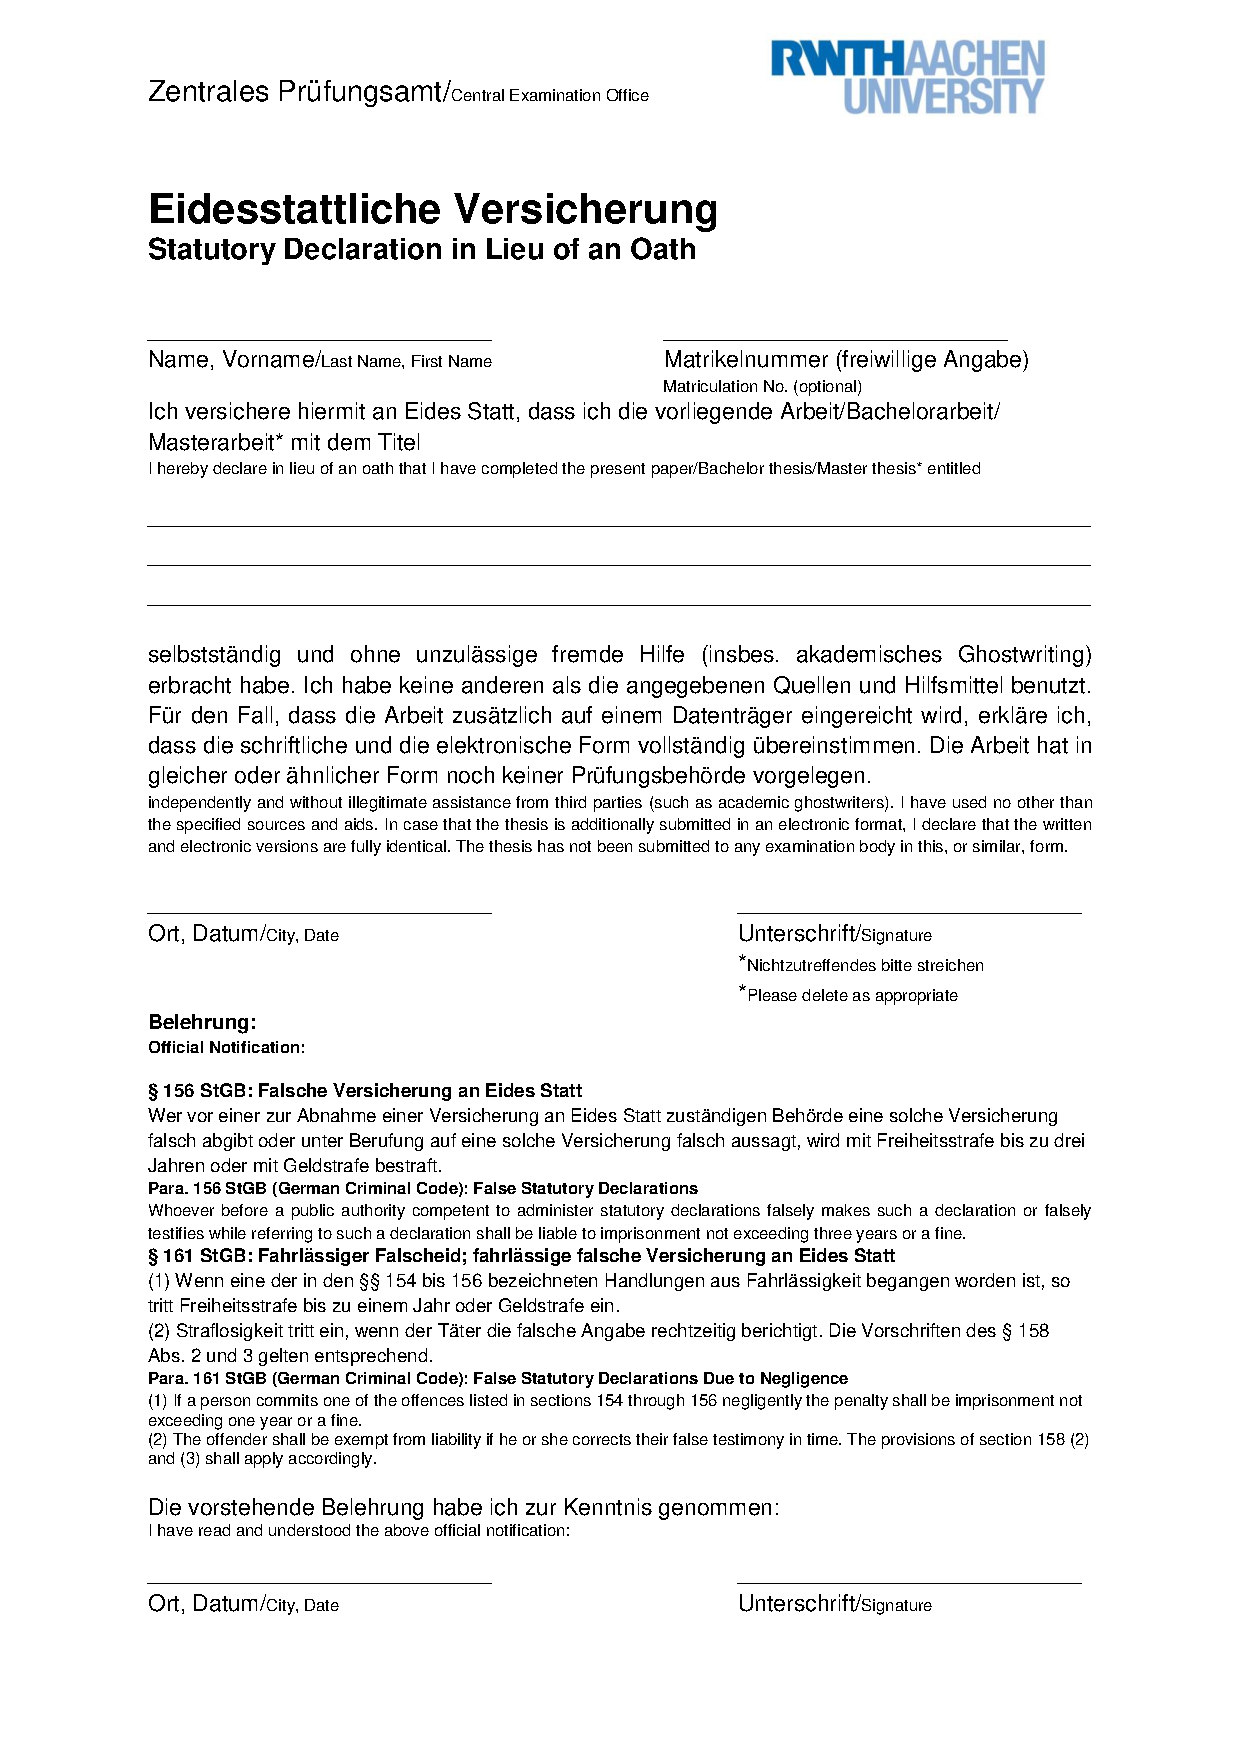
\includepdf[pages=-,pagecommand={},width=\textwidth]{files/oathstatement.pdf}

\end{document}
